%% main.tex --- Paper 1 (Semantic-communication effectiveness), TGCN edition.
%% Target venue: IEEE Transactions on Green Communications and Networking.
%% "Ask Before You Transmit: An Energy-Frugal Evidence-Level Semantic
%%  Communication System for UAV Visual Question Answering."
%% Submission format: single column, double spaced, 12 pt, <= 30 pages.
%% Compile: latexmk -pdf -outdir=build main.tex   (or pdflatex x2 + bibtex)

\documentclass[12pt,lettersize,journal,onecolumn]{IEEEtran}
% Class options follow the official TGCN initial-submission sample
% (bare_jrnl_new_sample4.tex): 12 pt, letter-size paper, journal mode,
% single column; double spacing via setspace below, as in the sample.
% (Older IEEEtran V1.8b releases report `lettersize' as an unused global
% option; letter paper is their default, so the layout is identical.)

% --------------------------------------------------------------------------
% Packages --- ordered as in the TGCN sample preamble, followed by the
% packages this manuscript additionally requires.
% --------------------------------------------------------------------------
% Template-mandated set (bare_jrnl_new_sample4.tex / New_IEEEtran_how-to):
\usepackage{amsmath,amsfonts}
\usepackage{algorithmic}
\usepackage{algorithm}
\usepackage{array}
\usepackage{textcomp}
\usepackage{url}
\usepackage{graphicx}
\usepackage{cite}
\hyphenation{op-tical net-works semi-conduc-tor IEEE-Xplore}
% Manuscript-required additions (theorems, tables, macros, review spacing):
\usepackage[T1]{fontenc}
\usepackage{amssymb,amsthm}
\usepackage{booktabs}
\usepackage{multirow}
\usepackage{xcolor}
\usepackage{xspace}
\usepackage{setspace}
\doublespacing % TGCN review format (single column, double spaced)
% Floats (tables/figures + captions) stay single-spaced, standard for
% review-format submissions; body text remains double-spaced.
\usepackage{etoolbox}
\AtBeginEnvironment{table}{\singlespacing}
\AtBeginEnvironment{figure}{\singlespacing}
% Float-placement tuning: avoid stranded bottom whitespace on pages that
% carry a top float (page budget; standard IEEE values are stricter).
\renewcommand{\topfraction}{0.95}
\renewcommand{\bottomfraction}{0.6}
\renewcommand{\textfraction}{0.05}
\renewcommand{\floatpagefraction}{0.9}
\setcounter{topnumber}{4}
\setcounter{totalnumber}{6}
% Tighter float/caption separation (page budget; floats are single-spaced
% while the body is double-spaced, so the stock 20pt gaps read oversized).
\setlength{\textfloatsep}{8pt plus 2pt minus 3pt}
\setlength{\floatsep}{6pt plus 2pt minus 2pt}
\setlength{\dbltextfloatsep}{8pt plus 2pt minus 3pt}
\setlength{\dblfloatsep}{6pt plus 2pt minus 2pt}
\setlength{\abovecaptionskip}{4pt}
\usepackage{hyperref}
% Submission style: keep hyperlinks functional but typeset in black.
\hypersetup{colorlinks=true,linkcolor=black,citecolor=black,urlcolor=black}

% --------------------------------------------------------------------------
% Custom macros
% --------------------------------------------------------------------------
\newcommand{\eg}{e.g.,\xspace}
\newcommand{\ie}{i.e.,\xspace}
\newcommand{\etal}{\textit{et al.}\xspace}
\newcommand{\sz}[1]{s_{#1}}
\newcommand{\TODO}[1]{\textcolor{red}{[TODO: #1]}}
\newcommand{\CITE}[1]{\textcolor{red}{[CITATION NEEDED: #1]}}

% Visible placeholder box for figures whose PDF asset is not yet under figures/.
% The \IfFileExists guard lets the document compile with or without the asset.
% \evfigw scales figure widths for the single-column review layout (a factor
% of 1.0 maps to ~0.5 text width; the length must be set at \AtBeginDocument
% time---in the preamble \linewidth is not yet the final text width, which
% silently collapsed every \evfig figure to a dot in earlier builds).
\newlength{\evfigw}
\AtBeginDocument{\setlength{\evfigw}{0.46\linewidth}}
\newcommand{\evfig}[4]{% {file}{width}{caption}{label}
  \begin{figure}[t]\centering
    \IfFileExists{figures/#1}{\includegraphics[width=#2\evfigw]{figures/#1}}%
      {\fbox{\parbox[c][4.5cm][c]{#2\evfigw}{\centering
        \textcolor{red}{\textbf{[\texttt{\detokenize{#1}} --- place PDF under figures/]}}}}}
    \caption{#3}\label{#4}
  \end{figure}}

% Theorem environments for the evidence-routing theory in Section V.
\newtheorem{proposition}{Proposition}
\newtheorem{lemma}{Lemma}
\newtheorem{corollary}{Corollary}
\newtheorem{remark}{Remark}
\newtheorem{definition}{Definition}

\begin{document}

% --------------------------------------------------------------------------
% Front matter
% --------------------------------------------------------------------------
\title{Ask Before You Transmit: An Energy-Frugal\\
Evidence-Level Semantic Communication System\\
for UAV Visual Question Answering}

% Author order (Zhang, Liu, Qin, Liang, da Fonseca): H. Liang after
% Z. Qin, per the corresponding author's instruction of 2026-09.
\author{Qiankun Zhang,
        Yue Liu,~\IEEEmembership{Member,~IEEE,}
        Zhijin Qin,~\IEEEmembership{Senior Member,~IEEE,}
        Hongbin Liang,~\IEEEmembership{Member,~IEEE,}
        and~Nelson~L.~S.~da~Fonseca,~\IEEEmembership{Senior Member,~IEEE}
\thanks{Manuscript submitted September~2026. \emph{(Corresponding author: Yue Liu.)}}
\thanks{Q.\ Zhang and Y.\ Liu are with the Faculty of Applied Sciences,
Macao Polytechnic University, Macao SAR, China
(e-mail: yue.liu@mpu.edu.mo).}
\thanks{Z.\ Qin is with the Department of Electronic Engineering, Tsinghua
University, Beijing, China.}
\thanks{H.\ Liang is with the School of Transportation and Logistics,
Southwest Jiaotong University, Chengdu, China
(e-mail: hbliang@swjtu.edu.cn).}
\thanks{N.\ L.\ S.\ da Fonseca is with the Institute of Computing, State
University of Campinas (UNICAMP), Campinas 13083-852, Brazil
(e-mail: nfonseca@ic.unicamp.br).}}

\markboth{IEEE Transactions on Green Communications and Networking (submitted)}%
{Zhang \MakeLowercase{\textit{et al.}}: Energy-Frugal Evidence-Level Semantic Communication for UAV VQA}

\maketitle
% IEEEtran.bst control: force "et al." beyond 6 authors (review page budget).
\bstctlcite{BSTcontrol}

% --------------------------------------------------------------------------
% Abstract
% --------------------------------------------------------------------------
\begin{abstract}
Uploading aerial images from an unmanned aerial vehicle (UAV) to an
edge vision--language model (VLM) enables visual question answering,
but image transmission and model inference incur energy costs for
every query. This paper proposes an evidence-level semantic
communication system for structured aerial visual question answering.
The transmitter selects either detection records or an image,
and the receiver uses a symbolic decoder or a frozen VLM,
respectively. A training-free question-type rule selects evidence
according to the information needed for the answer. A per-sample
router predicts branch correctness from sender-side features, while
an energy price adjusts the accuracy--energy trade-off. Evaluation
uses two aerial datasets and separates transmission, onboard
detection, and edge inference costs. Across three channel models
on VisDrone, the type rule improves accuracy over fixed-image
transmission and reduces accounted system energy by about $55\%$.
On DroneVehicle, a validation-selected learned router attains
$74.60\%$ accuracy at $4.47$ J per query, compared with $72.93\%$
at $11.21$ J for the type rule. Matched-receiver comparisons show
that adaptation can help, but nonlinear routing is not uniformly
better than a linear reference. The results support selecting
both evidence and answering computation according to the task.
The energy gains apply to the stated combined UAV-and-edge model,
not to measured UAV endurance.
\end{abstract}

\begin{IEEEkeywords}
Energy efficiency, evidence-level routing, semantic communication,
unmanned aerial vehicles, vision--language models, visual question answering.
\end{IEEEkeywords}

% --------------------------------------------------------------------------
% Body --- one \input{} per section.
% --------------------------------------------------------------------------
% Revised introduction: application, evidence trade-off, related approaches,
% specific gap, system overview, contributions, and organization.
\section{Introduction}\label{sec:intro}

\IEEEPARstart{U}{nmanned} aerial vehicles (UAVs) provide imagery for
inspection, traffic monitoring, and disaster assessment. Extracting useful
information from these images has motivated both human-assisted analysis
and automated object detection~\cite{ofli2016combining,pi2020convolutional}.
Visual question answering (VQA) offers another interface: users ask about
image content in natural language, such as the number of vehicles in a
scene. Remote sensing VQA has established this task and provided
benchmarks for evaluating it~\cite{lobry2020rsvqa}. With pretrained
vision--language models (VLMs)~\cite{wang2024qwen2vl}, an edge server can
process an aerial image together with a question. Applying this approach
over a UAV uplink, however, requires attention to both communication and
computation costs. Image transmission uses limited wireless resources,
while generating each answer also requires model inference. Reducing
the energy per question therefore calls for a design that considers both
costs.

The information required to answer a question need not include the full
image. For example, detected object classes and counts may support a
comparison between the numbers of cars and buses. Such structured
information has a small payload and can be processed by simple rules.
However, a missed object cannot generally be recovered from the detector
output alone. An image preserves visual details that may help answer
questions about objects omitted by the detector, but requires more
transmission and receiver computation. Moreover, the additional details
do not guarantee that a particular VLM will answer every question more
accurately. The choice depends on the question, the available detector
evidence, and the performance of the two processing paths over the link.
A useful selection method must identify when the smaller representation
is adequate and when image transmission is worth its cost.

Semantic and task-oriented communication provides the basis for making
such decisions according to the information needed by the receiver
task~\cite{gunduz2023beyond,strinati2021sixg,kountouris2021semantics}.
For wireless VQA, MU-DeepSC jointly designs the transceiver to convey
image and question features~\cite{xie2022mudeepscwcl}.
Goal-oriented VQA communication instead extracts and ranks bounding boxes
or scene-graph information according to the question~\cite{liu2024gosg}.
Query-oriented image coding also uses the query to select features for
image reconstruction~\cite{huang2026query}. Park and
Yoon~\cite{park2025transmit} compare visual representations across tasks
and select simpler or richer semantics according to task requirements.
Their task-level choice motivates examining which evidence and decoder
to use for each question within a VQA workload.
Du \etal~\cite{jiang2025lmmvn} use LLaVA for vehicle VQA and prioritize
image regions and patch transmission according to user interest.
That approach adapts the visual input to a multimodal model; our question
is when structured evidence can instead support symbolic decoding and
avoid VLM inference.
These studies establish task- and question-aware transmission as existing
design principles. In visual
reasoning, Prompt-RSVQA converts extracted visual context into text for a
language model~\cite{chappuis2022promptrsvqa}. Thus, structured visual
information is also an established alternative input to a reasoning
model.

A complementary line studies the energy implications of semantic
processing. Green semantic communication considers communication and
computation costs in aerial edge networks and probabilistic semantic
systems~\cite{zheng2024aerialee,dai2025pscom}. Input-aware VLM routing
selects between edge and cloud models according to the input and their
accuracy--cost trade-off~\cite{sabanovic2026inarvl}. Building on these
directions, we investigate a specific decision for structured aerial VQA:
whether to transmit detector information for symbolic decoding or an image
for VLM inference. The decision changes both the transmitted
representation and the computation needed to answer the question.
Its value must therefore be assessed through answer accuracy and the
combined communication and computation energy, rather than payload size
alone.

To study this decision, we propose an evidence-level semantic
communication system with a sender-side router and two receiver paths.
The token path transmits structured detector outputs and uses a
lightweight symbolic decoder. The image path transmits an image to a
frozen VLM. The system uses an aerial-domain detector and conventional
channel coding without jointly training the transceiver and the VLM.
A training-free rule selects the path from the question type. A learned
per-sample router further uses detector information to predict which path
will answer correctly, and an energy price controls the
accuracy--energy trade-off. We evaluate these choices on structured
questions about detected object categories. The aim is to identify when
evidence selection improves energy efficiency without reducing answer
accuracy, and to characterize the conditions under which the gain holds.
The main contributions are as follows:

\begin{itemize}
\item We formulate evidence selection as a joint choice of payload and
  receiver processing. The energy account includes transmission,
  onboard detection, and receiver inference, with UAV and edge costs
  distinguished. This formulation makes the cost of each answering path
  explicit and supports energy--accuracy comparisons.
\item We develop a training-free type rule and an MLP-based per-sample
  router. Conditional analysis explains when the type rule
  preserves accuracy while reducing energy. An energy-price extension
  provides a tunable operating point for the learned selector.
\item We evaluate the system on two aerial datasets, with AWGN,
  Rayleigh, and Rician channels on the primary dataset and Rician on
  the second. Evaluation combines logged-outcome replay, GPU power
  measurements, and transmission cost modeling. Under the reference
  configuration, the type rule reduces mean accounted energy per question by
  approximately $55\%$ on VisDrone relative to rate-adaptive image
  transmission while improving accuracy. On DroneVehicle, a
  validation-selected learned router achieves $74.60\%$ accuracy
  at $4.47$ J per query, compared with $72.93\%$ at $11.21$ J
  for the type rule. We retain simple baselines and matched-receiver
  comparisons to identify where learned selection helps and where
  its additional complexity offers little benefit. These results
  concern system energy, not a measured UAV battery gain.
\end{itemize}

The remainder of this paper is organized as follows.
Section~\ref{sec:related} reviews related work.
Section~\ref{sec:system} presents the system model and energy accounting.
Section~\ref{sec:routing} develops the selectors and their analytical
support. Section~\ref{sec:exp} reports the experiments and discusses
their limitations. Section~\ref{sec:conc} concludes the paper.

% Related work grouped by energy accounting, visual transmission, and
% adaptive inference. Comparisons identify decision variables and decoders.
\section{Related Work}\label{sec:related}

\subsection{Energy-Efficient Semantic Communication}
Energy-efficient semantic communication considers the cost of extracting
and processing information as well as transmitting it.
Zheng \etal~\cite{zheng2024aerialee} study aerial-aided edge networks
and develop incentive and distributed learning mechanisms for semantic
transmission and coder updates. PSCom~\cite{dai2025pscom} minimizes
communication and computation energy under constraints on latency,
power, bandwidth, and semantic compression. Rate-splitting designs
jointly allocate communication resources and semantic compression
levels~\cite{xu2025rsmagreen}. Related formulations address UAV networks,
including flight energy~\cite{wang2026rsma}, and visible-light systems
with knowledge-update overhead~\cite{zhao2026vlc}. These studies show
why savings in transmitted data must be evaluated together with the
computational cost of semantic processing.

For VLM-based services, the inference workload also affects the energy
account. Li \etal~\cite{li2026onboard} consider onboard VQA and optimize
image resolution, transmission power, and UAV trajectory under accuracy
constraints. Device-level measurements by Zhan
\etal~\cite{zhan2026seeing} identify autoregressive output generation
as a major energy cost in the VLM configurations they evaluate. Their
results indicate that reducing visual input alone may provide limited
inference-energy savings. These findings motivate accounting for the
processing required after transmission. Our study evaluates a
representation choice that also changes the answering computation:
symbolic decoding for detector information or VLM inference for an image.
UAV-side and edge-side costs are distinguished because they draw on
different energy supplies.

\subsection{Task-Oriented Visual Communication}
Learned image transmission provides one way to reduce communication
cost. Deep joint source--channel coding (DJSCC) maps images directly to
channel symbols and reconstructs them at the
receiver~\cite{bourtsoulatze2019djscc}. Attention-based coding adapts
to channel conditions~\cite{yang2023adjscc}, while predictive adaptive
coding uses estimated reconstruction quality to select the transmission
rate~\cite{zhang2023padc}. These methods improve the delivery of an
image representation. Task-oriented schemes additionally use the
requirements of the downstream task to determine what should be sent.

For wireless VQA, MU-DeepSC learns correlated image and question
representations with a jointly designed
transceiver~\cite{xie2022mudeepscwcl,xie2021mudeepsc}.
Goal-oriented VQA communication ranks bounding boxes and scene-graph
triplets using the question and employs an answer
reasoner~\cite{liu2024gosg}. Its comparison of representations across
question categories is directly relevant to evidence selection.
VideoQA-SC uses bandwidth-adaptive coding to answer video questions
from transmitted semantics without reconstructing the
video~\cite{guo2025videoqasc}. These approaches already evaluate
communication through the quality of the resulting answers, rather
than requiring accurate pixel reconstruction.

Other work adapts the representation or its protection to the task.
Park and Yoon~\cite{park2025transmit} compare object information,
layouts, and scene graphs across visual tasks and filter redundant
graph content. TONIC~\cite{liu2026tonic} assigns unequal protection
according to token relevance and combines receiver-side gating with
token completion for image classification. With pretrained multimodal
models, query-oriented coding selects features for query-relevant image
reconstruction~\cite{huang2026query}, and Du
\etal~\cite{jiang2025lmmvn} prioritize image regions and patch
transmission for a LLaVA-based vehicle assistant. These works motivate
task-dependent representation and transmission choices. The specific
choice examined here is between two complete answering paths within
a structured VQA workload. Each path has its own representation,
decoder, accuracy, and energy cost. Consequently, a smaller payload
may save both transmission energy and VLM inference, depending on
which decoder answers the question.

\subsection{Adaptive Inference and Evidence Selection}
Adaptive inference changes where computation takes place or how much
information reaches the server. Neurosurgeon~\cite{kang2017neurosurgeon}
partitions neural-network execution between a mobile device and the
cloud to reduce latency and mobile energy consumption. Information-bottleneck
methods learn compact representations for task-oriented edge
inference~\cite{shao2022taskoriented}. For VQA, INAR-VL
uses image and text complexity signals to route requests between
complementary edge and cloud VLMs~\cite{sabanovic2026inarvl}.
This provides an input-dependent choice of model and execution location.

Adaptive evidence delivery offers a related control variable.
Song and Kim~\cite{song2026collaborative} first send a thumbnail for
server-side VLM inference. The server uses output uncertainty to decide
whether to request an additional image region. Progressive semantic
communication compresses visual tokens into refinable representations
that can be supplied to off-the-shelf VLMs at different communication
budgets~\cite{hsu2026progressive}. SAGE~\cite{choi2026sage} selects
complementary visual evidence under a hard uplink budget and evaluates
the resulting classification accuracy. In remote sensing VQA,
Prompt-RSVQA converts extracted visual context into text for a language
model~\cite{chappuis2022promptrsvqa}. Thus, adaptive evidence selection
and structured context are established ways to support inference.

Our design combines sender-side evidence selection with a choice of
answering mechanism. It selects detector tokens for a symbolic decoder
or an image for a frozen VLM before transmitting the selected payload.
The decision does not require an initial receiver VLM pass or a request
for additional evidence. We assess its energy--accuracy trade-off using
logged-outcome replay, GPU power measurements, and models of transmission
and onboard detection costs. This distinguishes evidence-level routing
from model-placement decisions and from adapting the input to a VLM
that still runs on every query.

% System definition and accounting; evaluation details are in Section V.
\section{System Model}\label{sec:system}

\subsection{Network and Query Model}
A UAV captures an aerial image, and an edge server answers a question
about the observed scene. The UAV selects either structured detection
evidence or an image for transmission. The edge server then applies
the corresponding decoder, as shown in Fig.~\ref{fig:arch}. The
objective is to answer the question with low communication and
computation energy, rather than to maximize image reconstruction quality.

Let $I$ denote the source image and $q$ the question. We consider five
structured question types: presence, counting, comparison, co-presence,
and threshold. The model assumes that the question and its type are
available before evidence selection. Query delivery and parsing are
outside the communication and computation budget considered here.
The type rule uses only the question type. Other selectors may also
use an assumed SNR bin or features extracted from the image, as
specified in Section~\ref{sec:routing}.

Each image--question pair is treated as a separate transaction, with
no amortization of detection or transmission across questions. The
evaluation uses aerial images and recorded inference outcomes; it
does not include video scheduling or a live UAV control loop.

\begin{figure*}[!t]\centering
\fbox{\parbox{0.89\linewidth}{\centering
Image and question $\longrightarrow$ sender-side evidence selection\\[5pt]
\begin{tabular}{ccl}
Detection records & $\longrightarrow$ wireless link $\longrightarrow$ & Symbolic decoder\\[3pt]
JPEG image & $\longrightarrow$ wireless link $\longrightarrow$ & Frozen VLM
\end{tabular}\\[5pt]
One selected payload and one receiver answering path per query}}
\caption{Evidence-level routing jointly selects the transmitted
representation and receiver computation. The type rule decides
before detection; the per-sample router first extracts detector
features. Neither policy requires an initial receiver VLM pass.}\label{fig:arch}
\end{figure*}

\subsection{Evidence Representation and Answer Generation}
\label{subsec:levels}\label{subsec:answering}
The detection-evidence branch uses an onboard
YOLOv8n detector~\cite{jocher2023yolov8} to extract
\begin{equation}
Z=g(I)=\{(c_j,b_j,p_j)\}_{j=1}^{J},
\end{equation}
where $J$ is the number of detected objects, and $c_j$, $b_j$, and
$p_j$ are the class label, bounding box, and confidence of object $j$.
These records form a symbolic packet. The receiver applies
question-specific count and logical operations to the received
evidence $\tilde Z$. No neural inference is required at the receiver
on this branch; neural detection is performed on the UAV.

The image branch transmits a JPEG representation of $I$. The
reconstructed image $\hat I$ and question $q$ are passed to a frozen
Qwen2-VL-2B model~\cite{wang2024qwen2vl}. The model generates the
answer by greedy decoding. Thus, evidence selection changes both the
transmitted representation and the computation used to answer the
question. Writing $s\in\mathcal{S}=\{\mathrm{det},\mathrm{img}\}$ for
the selected branch, the answer is
\begin{equation}\label{eq:answer}
\hat A_q=
\begin{cases}
D_{\mathrm{sym}}(\tilde Z,q), & s=\mathrm{det},\\[2pt]
D_{\mathrm{VLM}}(\hat I,q), & s=\mathrm{img},
\end{cases}
\end{equation}
where $D_{\mathrm{sym}}$ and $D_{\mathrm{VLM}}$ denote the symbolic
decoder and the VLM, respectively. Detector training, count
calibration, and answer scoring are described in
Section~\ref{subsec:setup}.

\subsection{Channel and Transmission Model}\label{subsec:phy}
\label{subsec:channels}
The uplink is represented by a normalized flat-fading channel,
\begin{equation}\label{eq:link}
y=hx+n,\qquad n\sim\mathcal{CN}(0,\sigma_n^2),
\end{equation}
with $\mathbb{E}[|x|^2]=1$ and $\mathbb{E}[|h|^2]=1$.
The average received SNR is $\gamma=1/\sigma_n^2$, and the
instantaneous SNR is $\gamma|h|^2$. We consider AWGN ($h=1$),
Rayleigh ($h\sim\mathcal{CN}(0,1)$), and Rician fading. For Rician
fading,
\begin{equation}
h=\sqrt{\frac{K}{K+1}}h_{\mathrm{LoS}}
 +\sqrt{\frac{1}{K+1}}h_{\mathrm{NLoS}},
\end{equation}
where $|h_{\mathrm{LoS}}|=1$,
$h_{\mathrm{NLoS}}\sim\mathcal{CN}(0,1)$, and $K$ is the linear
line-of-sight to scattered-power ratio. These models represent
different propagation conditions relevant to air-to-ground
links~\cite{khawaja2019survey}. Distance and path loss are absorbed
into the received SNR; UAV geometry and trajectory are not optimized.

\emph{Detection-evidence transmission.}\label{subsec:detphy}
Let $L_{\mathrm{det}}$ denote the packet length in bits. Its nominal
airtime uses rate-$1/2$ low-density parity-check (LDPC)
coding~\cite{gallager1962ldpc} and binary phase-shift keying (BPSK).
The main evaluation approximates evidence loss through
\begin{equation}\label{eq:outage}
P_{\mathrm{out}}(\gamma)
=\Pr\!\left[\log_2(1+\gamma|h|^2)
 <\frac{L_{\mathrm{det}}}{B\tau}\right],
\end{equation}
where $B$ is the bandwidth and $\tau$ is a reference transmission
window. This is an information-outage abstraction, not the measured
frame error rate (FER) of a compact LDPC packet. Its single fading
gain does not describe coding across multiple independent fading
blocks~\cite{tse2005fundamentals}.

The evidence impairment model allows records to be dropped or
corrupted, with equal probabilities conditional on a loss event.
Surviving records form $\tilde Z$ for symbolic decoding. This is an
application-level corruption model, not a model of residual errors
after packet integrity checks. The resulting answer accuracy is
conditional on this impairment assumption.

\emph{Image transmission.}\label{subsec:imgphy}
The rate-adaptive image branch uses the ergodic spectral efficiency
\begin{equation}\label{eq:se}
\mathrm{SE}(\gamma)
=\mathbb{E}_{h}[\log_2(1+\gamma|h|^2)]
\end{equation}
as an idealized rate for airtime accounting~\cite{tse2005fundamentals}.
The image traces use channel-dependent JPEG quality and resolution.
Let $L_{\mathrm{img}}(I,\gamma)$ be the compressed payload length
in bits before receiver-side decoding and file storage. The codec
reduces JPEG quality and, if needed, image resolution to meet the
reference transmission window. A received image saved again as a
JPEG is not used to estimate the transmitted payload.
The accounting uses the recorded reconstruction $\hat I$ for answer
evaluation and does not establish that a finite-length LDPC code
achieves \eqref{eq:se}. On an outage, the model returns a gray
image and charges the full reference window; no successful source
encoding length is recorded for that event.

\emph{Airtime.}\label{subsec:accounting}
With one complex channel use per $1/B$ seconds, the compact-packet
and ideal-rate accounting conventions give
\begin{equation}\label{eq:uses}
\begin{aligned}
T_s(\gamma)&=\frac{u_s(\gamma)}{B},\\
u_{\mathrm{det}}&=2L_{\mathrm{det}},\qquad
u_{\mathrm{img}}(\gamma)=
\frac{L_{\mathrm{img}}(I,\gamma)}{\mathrm{SE}(\gamma)}.
\end{aligned}
\end{equation}
Dependence on the source image is suppressed in $T_s$ and $u_s$ for
brevity. The image expression applies to non-outage transmissions; on outage,
$T_{\mathrm{img}}=\tau$. The energy tables use these conventions.
The nominal compact-packet airtime is not jointly coupled to the
outage-based reliability in \eqref{eq:outage}; a joint finite-length
reliability and airtime evaluation is needed to establish that
operating point. We therefore distinguish modeled airtime from a
validated link-level latency guarantee.

\subsection{Energy and Latency Models}\label{subsec:energyacct}
We account for communication and computation energy per question,
following the joint accounting approach of~\cite{dai2025pscom}.
Let $\rho$ denote the selector, and let $d_\rho(s)$ indicate whether
the detector runs for the selected branch. Type-based selectors run
the detector only when sending detection evidence. Per-sample
selectors need detector features before making a choice, so their
detector runs for every query. The platform-specific costs are
\begin{equation}\label{eq:energy}
\begin{aligned}
E_\rho^{\mathrm{UAV}}(s,\gamma)
 &=\frac{P_{\mathrm{tx}}}{\eta}T_s(\gamma)
   +d_\rho(s)E_{\mathrm{det}}\\
 &\quad+E_{\mathrm{route},\rho}+E_{\mathrm{enc}}(s),\\
E^{\mathrm{edge}}(s)
 &=\begin{cases}
 E_{\mathrm{sym}}, & s=\mathrm{det},\\
 E_{\mathrm{VLM}}, & s=\mathrm{img},
 \end{cases}\\
E_\rho(s,\gamma)
 &=E_\rho^{\mathrm{UAV}}(s,\gamma)+E^{\mathrm{edge}}(s).
\end{aligned}
\end{equation}
Here $P_{\mathrm{tx}}$ is radiated power, $\eta$ is power-amplifier
efficiency, and $E_{\mathrm{enc}}$ covers source encoding beyond
detector execution. $E_{\mathrm{det}}$, $E_{\mathrm{route},\rho}$,
$E_{\mathrm{sym}}$, and $E_{\mathrm{VLM}}$ denote detector, routing,
symbolic-decoding, and VLM-inference energy. The reference account
uses $\eta=1$. The efficiency term permits amplifier losses to be
included as in~\cite{cui2005energy}, but the reported comparisons
use the reference efficiency. Transmit power and the link budget
are not jointly optimized.

VLM energy is measured on an RTX~4060 edge-server proxy. Onboard
detector energy is modeled using a Jetson-class power and latency
range, with a separate desktop measurement as a cross-check.
Routing, symbolic decoding, and image source encoding are assigned
zero energy in the reported account; these are exclusions, not
measurements of zero consumption. Omitting image encoding reduces
the charged cost of the image branch. It does not bound all omitted
system costs. Numerical settings are given in
Section~\ref{subsec:energy-exp}.

For sequential execution, the corresponding per-question latency is
\begin{equation}\label{eq:latency}
\begin{aligned}
T_\rho^{\mathrm{total}}(s,\gamma)
 &=d_\rho(s)T_{\mathrm{det}}^{\mathrm{cmp}}
   +T_{\mathrm{route},\rho}^{\mathrm{cmp}}
   +T_{\mathrm{enc}}^{\mathrm{cmp}}(s)\\
 &\quad+T_s(\gamma)+T_{\mathrm{ans}}^{\mathrm{cmp}}(s),
\end{aligned}
\end{equation}
where the superscript $\mathrm{cmp}$ distinguishes processing time
from airtime. Answer processing is symbolic decoding or VLM
inference, according to the selected branch. Queueing and inter-query
overlap are not modeled. If transmission occupies the full reference
window, end-to-end latency also includes processing time and therefore
exceeds $\tau$.

The main account uses over-idle inference energy for an unbatched,
dedicated edge server.
Flight, image acquisition, control signaling, and radio circuitry
outside the amplifier model are excluded. Total accounted energy
includes both platforms, but UAV battery savings depend on the net
change in $E_\rho^{\mathrm{UAV}}$, including onboard computation.
Avoided edge inference does not directly extend UAV battery life.

% Section IV: type rule, learned per-sample routing, and conditional analysis.
\section{Question-Conditioned Evidence Routing}\label{sec:routing}

The two branches in Section~\ref{sec:system} differ in both the
information they transmit and the computation they require. Evidence
routing selects a branch before transmission. When detection evidence
is sufficient to answer the question, the receiver can avoid VLM
inference. We first introduce a question-type rule that requires no
router training. We then develop a per-sample router that uses the
current detector output to refine branch selection. The final subsection
analyzes the conditions under which evidence selection can reduce
energy without reducing accuracy.

\subsection{Question-Type-Based Evidence Selection}\label{subsec:rule}

Counting, comparison, co-presence, and threshold questions can be
expressed as functions of object counts. The detection-evidence branch
provides these counts to a symbolic decoder and avoids image-based
inference at the receiver. Presence questions can also be answered
from detections. However, a failure to detect an object does not mean
that the object is absent from the scene. The image branch retains
visual information that the detector may have missed. This difference
motivates branch selection based on question type.

Let $t(q)$ denote the type of question $q$. Let
$\mathcal T_{\mathrm{sym}}$ contain counting, comparison, co-presence,
and threshold, and let $\mathcal T_{\mathrm{pres}}$ contain presence.
The type rule is
\begin{equation}
r(t(q))=
\begin{cases}
\mathrm{det}, & t(q)\in\mathcal T_{\mathrm{sym}},\\
\mathrm{img}, & t(q)\in\mathcal T_{\mathrm{pres}}.
\end{cases}
\label{eq:rule}
\end{equation}
The rule uses neither channel-state information (CSI) nor receiver
feedback. If it selects the detection-evidence branch, the UAV runs
the detector and transmits the resulting packet. Otherwise, it
transmits the image without running the detector for routing. Thus,
the decision also determines whether onboard detection is required.
Equation~\eqref{eq:energy} includes this detection cost.

Equation~\eqref{eq:rule} defines a fixed rule. It does not guarantee
that the selected branch is more accurate for every question of a
given type. Missed objects, false detections, and image distortion can
change which evidence is more useful for an individual query.
For threshold questions, detection errors can move the estimated count
across the threshold specified in the question and change the answer. A type-only
rule cannot account for these sample-specific differences. This
motivates the learned router below.

\subsection{Per-Sample Evidence Routing}\label{subsec:persample}

The per-sample router predicts whether each branch will answer correctly
using information available before transmission. For each query, the
UAV first computes $Z=g(I)$ and constructs a feature vector $x$.
The feature vector has $18$ entries: five question-type indicators,
ten target-class indicators, the assumed SNR in dB divided by $20$,
the target-class detection count clipped at $60$ and divided by $60$,
and an indicator of whether that count is nonzero. The count is
computed from the original detector records $Z$, before channel
impairment. It is not the count recovered at the receiver.
Ground-truth answers, annotation-derived scene attributes, and
receiver outputs are excluded. The assumed SNR is a transmitter-side
input; no receiver VLM pass is required before selection.

For each branch $s\in\mathcal S=\{\mathrm{det},\mathrm{img}\}$, let
$\widehat p_s(x)$ estimate the probability that its answer is correct.
Training uses paired binary labels $y_{i,s}\in\{0,1\}$ from the
recorded answers of both branches. Each pair corresponds to the same
image, question, and channel condition. Each label indicates whether
the answer meets the scoring rule in Section~\ref{subsec:setup}.
The labels describe the correctness of each branch, rather than
identify one preferred branch. Both answers can therefore be correct
or incorrect.

We train the correctness predictors using binary cross-entropy.
For $N_{\mathrm{tr}}$ training decisions, the data-fitting term is
\begin{equation}
\mathcal L_{\mathrm{BCE}}
=-\frac{1}{2N_{\mathrm{tr}}}
\sum_{i=1}^{N_{\mathrm{tr}}}\sum_{s\in\mathcal S}
\left[y_{i,s}\log\widehat p_s(x_i)
+(1-y_{i,s})\log(1-\widehat p_s(x_i))\right].
\label{eq:router-loss}
\end{equation}
We use compact multilayer perceptron (MLP) predictors.
Each predictor has two hidden layers with $32$ and $16$ units and
uses ReLU activations. We train the predictors with Adam.
Predictor fitting uses training images, and early stopping uses a
separate set of validation images. All questions and SNR replays of
an image stay in the same partition. Section~\ref{subsec:setup}
specifies the split, count calibration, and repeated runs.
Predicting branch performance before transmission is related to
predictive adaptation in image semantic communication~\cite{zhang2023padc}.
Here, the prediction target is answer correctness rather than image
reconstruction quality.

The default decision selects the branch with the higher predicted
probability of a correct answer:
\begin{equation}
\widehat s(x)=\arg\max_{s\in\mathcal S}\widehat p_s(x).
\label{eq:argmax}
\end{equation}
An energy-aware extension uses the same predictors and includes a
weighted energy cost in the decision:
\begin{equation}
\widehat s_\lambda(x)=
\arg\max_{s\in\mathcal S}
\left[\widehat p_s(x)-\lambda E_\rho(s,\gamma)\right],
\qquad \lambda\ge0,
\label{eq:argmax-lambda}
\end{equation}
where $\lambda$ has units J$^{-1}$ and $E_\rho(s,\gamma)$ is the
energy for selector $\rho$ in \eqref{eq:energy}. Setting $\lambda=0$
gives \eqref{eq:argmax}. We report this setting alongside
energy-aware operating points. A positive energy price favors the lower-cost branch when
its predicted accuracy is sufficiently close to that of the other
branch. Section~\ref{subsec:energyctl} evaluates a fixed price grid
and a validation-selected operating point. Costs are evaluated
per query; their image dependence is suppressed in the notation.
The rule does not impose a hard per-query budget or guarantee
a test-set accuracy loss.

Algorithm~\ref{alg:selector} summarizes the two routing options.
Unlike the type rule, per-sample routing runs the detector for every
query, even when it selects the image branch. This detection cost is
the same for both branch choices and does not change their score
difference. It must still be included in the total energy.
The selected branch then follows the transmission and
answer-generation models of Section~\ref{sec:system}. Training uses
paired outcomes, but inference transmits only the selected evidence.
The experiments evaluate this procedure by replaying recorded branch
outcomes rather than running a live control loop. The type-level
lookup table and linear predictor serve as baselines.
Section~\ref{subsec:setup} defines these baselines.

\begin{algorithm}[t]
\caption{Question-conditioned evidence routing for one query}
\label{alg:selector}
\begin{algorithmic}[1]
\REQUIRE image $I$; question $q$ and type $t(q)$; routing mode
$\rho\in\{\mathrm{rule},\mathrm{MLP}\}$;
for MLP, target class, assumed SNR $\gamma$, predictors
$\widehat p_s$, and energy price $\lambda$ (default $0$)
\IF{$\rho=\mathrm{rule}$}
  \STATE $\widehat s\leftarrow r(t(q))$ using \eqref{eq:rule}
\ELSE
  \STATE compute $Z=g(I)$ and construct features $x$
  \STATE predict $\widehat p_{\mathrm{det}}(x)$ and $\widehat p_{\mathrm{img}}(x)$
  \STATE select $\widehat s$ using \eqref{eq:argmax-lambda}
\ENDIF
\IF{$\widehat s=\mathrm{det}$}
  \IF{$\rho=\mathrm{rule}$}
    \STATE compute $Z=g(I)$
  \ENDIF
  \STATE transmit $Z$; answer from received evidence $\widetilde Z$
\ELSE
  \STATE transmit the rate-adaptive coded image; answer from $\widehat I$
\ENDIF
\end{algorithmic}
\end{algorithm}

\subsection{Analysis of Evidence Selection}\label{sec:theory}

\emph{Information required by the question.}
Consider a counting question with ground truth $A_q=N_c(I)$.
If detection recovers the true count and transmission preserves the
relevant records, then
$\widehat N_c(\widetilde Z)=N_c(I)$, and
\begin{equation}
H\!\left(A_q\mid\widehat N_c(\widetilde Z)\right)=0.
\label{eq:count-sufficiency}
\end{equation}
Thus, under these ideal conditions, the detection evidence contains
all information needed for that answer. The image is not required.
The same result applies to comparison, co-presence, and
threshold questions when all relevant class counts are recovered.
This result states when detection evidence is sufficient. It does
not guarantee that a practical detector or a noisy link meets these
conditions.

In practice, the detection-evidence branch is affected by detection
errors and corruption or loss of transmitted records. The image
branch is affected by compression, channel degradation, and VLM
answering errors. For presence questions, an object missed by the
detector may be absent from the packet but still visible in the
image. This explains a potential advantage of
image transmission. It does not prove that the image branch is
always more accurate. The comparison depends on false positives, missed
objects, the channel, and the actual receiver. Section~\ref{subsec:comp}
therefore measures branch accuracy by question type instead of
inferring it from detector recall alone.

\emph{Conditions for energy reduction.}
\label{subsec:pareto-theory}
Fix a channel condition and the computation model. Let question type
$t\in\mathcal T$ have probability $w_t>0$, with
$\sum_{t\in\mathcal T}w_t=1$. Let $a_s(t)$ and $e_s(t)$ denote the
expected accuracy and per-query energy of branch $s$, respectively.
Here the costs correspond to type-only selection: detection is
performed only when its branch is selected. A deterministic
type-based policy $\pi:\mathcal T\to\mathcal S$ has
\begin{equation}
A(\pi)=\sum_{t\in\mathcal T}w_t a_{\pi(t)}(t),
\qquad
E(\pi)=\sum_{t\in\mathcal T}w_t e_{\pi(t)}(t).
\label{eq:policy}
\end{equation}

\begin{proposition}[Conditional energy--accuracy dominance]\label{prop:pareto}
Let $\mathcal T=\mathcal T_{\mathrm{sym}}\cup\mathcal T_{\mathrm{pres}}$,
where the two sets in \eqref{eq:rule} are disjoint and nonempty. Assume that
$e_{\mathrm{det}}(t)<e_{\mathrm{img}}(t)$ for every $t$, and that
\begin{equation}
\begin{aligned}
a_{\mathrm{det}}(t)&\ge a_{\mathrm{img}}(t),
&&t\in\mathcal T_{\mathrm{sym}},\\
a_{\mathrm{img}}(t)&>a_{\mathrm{det}}(t),
&&t\in\mathcal T_{\mathrm{pres}}.
\end{aligned}
\label{eq:ordering}
\end{equation}
Then the type rule $r$ maximizes $A(\pi)$ over deterministic type-based
policies. Among the policies with maximum accuracy, $r$ has the lowest
energy. Relative to the fixed-image policy $\pi_{\mathrm{img}}$,
it satisfies $A(r)\ge A(\pi_{\mathrm{img}})$ and
$E(r)<E(\pi_{\mathrm{img}})$.
\end{proposition}

\emph{Proof.}
Each term in the accuracy sum in \eqref{eq:policy} can be maximized
separately. Under \eqref{eq:ordering}, $r$ selects a branch with maximum
accuracy for each type. When the two branches have equal accuracy,
the detection-evidence branch has lower energy. On the symbolic
types, $r$ replaces image transmission with detection evidence without
reducing accuracy. These types have positive total probability, so
this replacement strictly reduces the expected energy.
These observations prove the stated results. \hfill$\square$

The proposition states sufficient conditions, not a general
optimality guarantee for \eqref{eq:rule}. In particular, the accuracy
condition must also hold for threshold questions, which are part of
$\mathcal T_{\mathrm{sym}}$. A small observed accuracy difference does
not establish equality or confirm this condition. The
experiments assess the rule and the learned router directly under
the stated energy model. The MLP uses information beyond question
type and has different computation costs. This proposition therefore
does not prove the gains measured for the MLP.

% Existing, provenance-checked outcomes only; no new experiment runs.
\section{Experiments and Discussion}\label{sec:exp}
We examine three questions: whether selecting evidence by question type
improves on transmitting the same representation for every query;
how per-sample prediction changes the accuracy--energy trade-off;
and whether a router remains useful when the receiver changes.
The evaluation separates these questions rather than assuming that
one routing policy is best in every setting.

\subsection{Experimental Setup}\label{subsec:setup}\label{subsec:tasks}
\emph{Datasets and splits.}
VisDrone-DET~\cite{zhu2021visdrone} provides $548$ aerial images,
and DroneVehicle~\cite{sun2022dronevehicle} provides $490$ images.
The questions cover presence, counting, comparison, co-presence,
and threshold. For image identifier $i$, we compute
$\mathrm{crc32}(i)\bmod100$. Values below $20$ define the test set,
values at least $80$ define validation, and the remaining values
define training. All questions and channel replays of an image
remain in one partition. VisDrone contains $343/101/104$
training/validation/test images; DroneVehicle contains $275/93/122$.
The test sets contain $936$ and $710$ questions, respectively.
Six SNR points yield $5{,}616$ decisions per VisDrone channel and
$4{,}260$ DroneVehicle decisions. Repeated log entries are deduplicated
by image, question, SNR, and branch.

The channel sweep compares fixed evidence, the type rule, and a
training-set lookup table (LUT) on VisDrone. Per-sample comparisons
use the verified AWGN records, the DroneVehicle target-data fit,
and the matched-receiver experiment below. These are distinct
evaluation settings, not interchangeable samples of one benchmark.
In particular, target-data fitting on DroneVehicle is not
VisDrone-to-DroneVehicle zero-shot transfer.

\emph{Answering and scoring.}
The YOLOv8n detector is trained on the official VisDrone training
split, disjoint from the evaluation images. It is not retrained on
DroneVehicle. The default image receiver is frozen
Qwen2-VL-2B~\cite{wang2024qwen2vl}, with greedy decoding and at most
$24$ generated tokens. The other branch applies symbolic operations
to the full received detection packet. Yes/no answers use exact
match after canonicalization. For counting, an estimate is correct
when its absolute error is at most
$\max(1,\operatorname{round}(0.1N))$, where $N$ is the true count.

Count calibration is fitted only on training images, by class and
SNR. The ratio of summed true to received training counts is clipped
to $[0.5,4]$ and retained only if it does not reduce training counting accuracy; counts below
three are left unchanged. The fitted ratios are frozen for validation
and test. An uncalibrated control is retained in the supplementary
materials. Calibration changes the receiver's counting answer, not
the sender's detector features. Learned inputs use pre-transmission
counts checked against the original detection records.

\emph{Channels and energy.}\label{subsec:energy-exp}
VisDrone uses AWGN, Rayleigh, and Rician channels at
$\{-5,0,5,10,15,20\}$\,dB; DroneVehicle uses Rician at the same SNRs.
The Rician factor is $K=6$\,dB. Bandwidth, reference window, and
radiated power are $1$\,MHz, $0.3$\,s, and $0.5$\,W.
The JPEG codec reduces quality, then resolution if necessary.
For cost reconstruction, the original codec and random seeds are
replayed on the source images. The resulting receiver JPEGs must
match the stored images byte for byte before their answers are
paired with recovered transmitted-payload costs.
All $9{,}864$ VisDrone image/SNR records and $2{,}940$
DroneVehicle image/SNR records pass this check. DroneVehicle also
passes checks on all $7{,}320$ recorded receiver-file paths.
Outages incur the full $0.3$\,s window. Detection-packet costs retain
the compact-airtime model in Section~\ref{subsec:phy}.

Table~\ref{tab:power} reports the GPU measurements underlying the
energy model. Edge VLM energy is the over-idle value of $32.31$\,J
per answer on an RTX~4060 proxy, measured on the $5$\,dB workload.
It is held fixed across the evaluated channel conditions and both
datasets, not measured anew on DroneVehicle. Sampling is approximately
$8$\,Hz over steady-state windows after a $20$\,s warm-up.
Onboard detector energy is modeled as $0.4275$\,J using a
Jetson-class power/latency envelope~\cite{nvidia2024orinnano};
it is not an embedded-device measurement. The reference amplifier
efficiency is $\eta=1$.

\begin{table}[t]\centering
\caption{GPU measurements. The detector desktop cross-check is not
the modeled onboard cost. VLM incremental energy is the reference
edge cost used in the analysis.}\label{tab:power}
\footnotesize
\begin{tabular}{@{}lrrrr@{}}\toprule
Phase & Power (W) & Time/item (s) & Incremental (J) & Total (J)\\
\midrule
Idle & 52.3 & --- & --- & ---\\
YOLOv8n cross-check & 58.7 & 0.0104 & 0.066 & 0.61\\
Qwen2-VL-2B & 107.9 & 0.581 & 32.31 & 62.72\\
\bottomrule\end{tabular}
\end{table}

Learned selectors pay detector energy for every query; the type
rule and LUT pay it only when selecting detection evidence.
Selected-sample airtime is used rather than a branch-wide mean
payload. Source encoding, router execution, symbolic decoding,
flight, sensing, queueing, and radio circuitry are excluded.
Savings therefore refer to the stated combined UAV-and-edge
account, not to measured UAV endurance.

\emph{Baselines and repeated runs.}\label{subsec:lcb}\label{subsec:stats}
The fixed-image and fixed-detection policies establish the two
answering paths. The type rule is training-free. The LUT chooses
a branch for each question-type/SNR cell using training accuracy,
with ties resolved toward detection. For paired branches with equal
sample counts this ranking is also the ranking of their Wilson
lower bounds~\cite{wilson1927probable}.
Linear routing uses two logistic correctness predictors with the
same inputs as the MLP. Its optimizer uses $400$ fixed steps,
step size $0.5$, and L2 coefficient $0.001$.
MLP hidden layers have $32$ and $16$ units; Adam uses learning rate
$0.001$, batch size $200$, and L2 coefficient $0.0001$.
Training stops after $10$ epochs without validation BCE improvement
of $10^{-4}$, with a $300$-epoch maximum, and restores the best
validation model. All MLP comparisons retain seeds $0$--$9$.

MLP results are means over these ten seeds; reported standard
deviations describe training-seed variation, not uncertainty across
independent datasets. SNR replays and questions sharing an image
are not independent observations. The comparisons below are
descriptive; small mean differences are not called statistically
significant. The supplementary materials give the provenance
boundary and additional verified controls.

\subsection{Question-Type Routing and Evidence Complementarity}
\label{subsec:main}\label{subsec:comp}\label{subsec:mechanism}
Figure~\ref{fig:f1} compares fixed evidence and type-based selection
over the VisDrone channel grid. The type rule reaches
$67.47\%$, $66.92\%$, and $67.27\%$ accuracy on AWGN, Rayleigh,
and Rician, respectively, after pooling the six SNRs.
The corresponding image accuracies are $60.43\%$, $60.15\%$,
and $60.63\%$. Thus, a simple change in answering path improves
accuracy without requiring a learned per-sample selector.

\begin{figure}[t]\centering
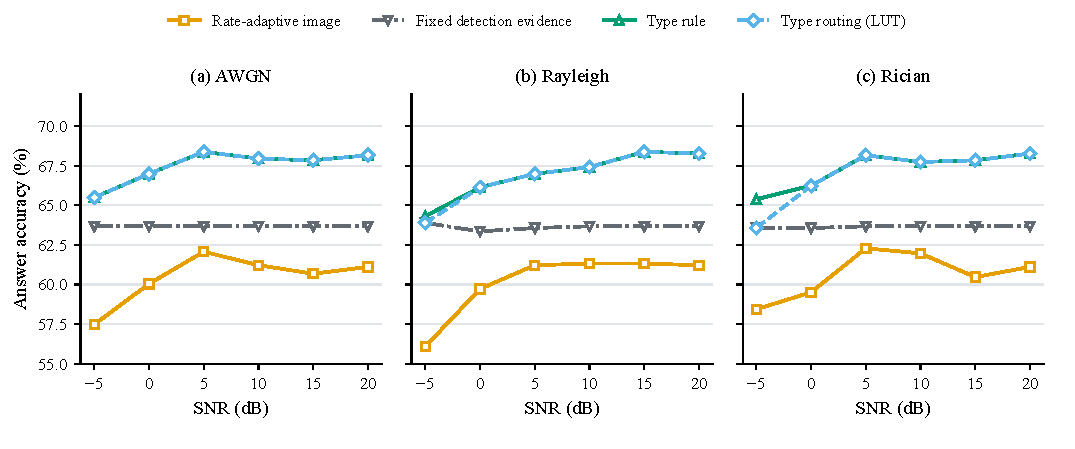
\includegraphics[width=\linewidth]{figures/evidence_final/type_routing.pdf}
\caption{VisDrone answer accuracy: $936$ questions per SNR,
with all five question types. These fixed-policy curves do not
have training-seed error bars. The LUT is fitted on training images
and is distinct from the fixed type rule.}\label{fig:f1}
\end{figure}

\begin{table}[t]\centering
\caption{VisDrone accuracy (\%) pooled over six SNRs.
Each channel contains $5{,}616$ decisions.}\label{tab:persample}
\footnotesize
\begin{tabular}{@{}lrrr@{}}\toprule
Policy & AWGN & Rayleigh & Rician\\\midrule
Image & 60.43 & 60.15 & 60.63\\
Detection evidence & 63.68 & 63.64 & 63.64\\
Type rule & 67.47 & 66.92 & 67.27\\
Training LUT & 67.47 & 66.84 & 66.97\\
\bottomrule\end{tabular}
\end{table}

The type rule uses approximately $14.46$\,J per query, compared
with $32.45$\,J for the image branch: a system saving of about
$55.4\%$. It routes $43.8\%$ of queries to the image receiver.
The LUT produces similar pooled accuracy, but chooses images less
often on the fading channels. Similar accuracy alone is therefore
not evidence that two policies have the same energy cost, nor does
it establish statistical equivalence.

Figure~\ref{fig:comp} explains why evidence selection can help.
On Rician VisDrone, detection evidence exceeds the image branch
by $18.07$, $13.62$, and $10.42$ percentage points for counting,
comparison, and co-presence. The image branch is better on presence
by $8.29$ points. Threshold is an exception to the symbolic-type
ordering: detection is lower by $1.44$ points. On DroneVehicle,
detection is better for all four count-based types, whereas the
presence gap favoring images is only $1.39$ points.
The branch ordering thus depends on the task and dataset.
These measurements motivate the rule but do not establish the
conditions of Proposition~\ref{prop:pareto} in every setting.

\begin{figure}[t]\centering
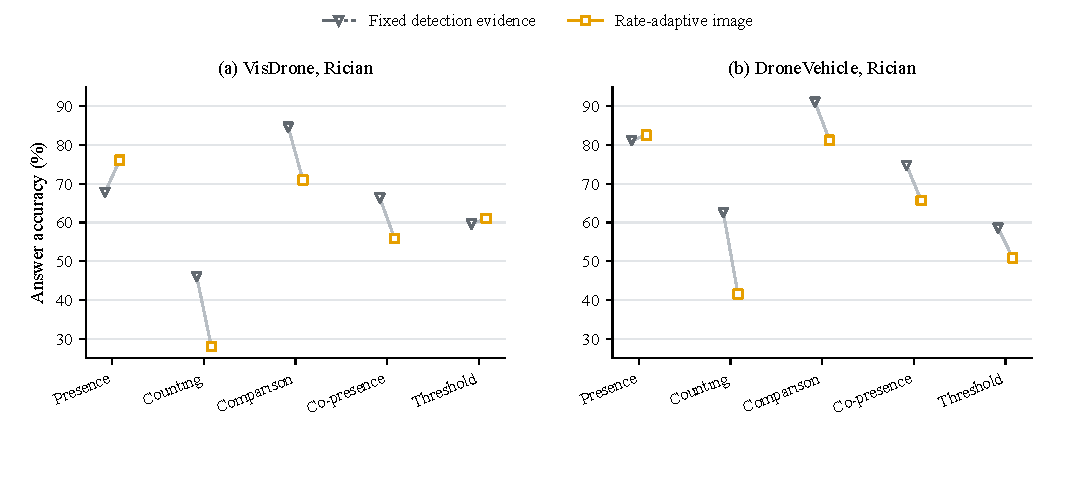
\includegraphics[width=\linewidth]{figures/evidence_final/evidence_complementarity.pdf}
\caption{Fixed-branch accuracy by question type, pooled over the
six Rician SNRs. The panels use their respective dataset questions;
they compare evidence within each dataset, not matched images
between datasets.}\label{fig:comp}
\end{figure}

\subsection{Per-Sample Routing and Energy Control}
\label{subsec:persample-exp}\label{subsec:energyctl}
A learned predictor can exploit sample differences within a question
type, but its value should be assessed against simple alternatives.
On the verified VisDrone AWGN evaluation, the unpriced MLP attains
$67.92\%\pm0.19\%$ accuracy at $13.38$\,J per query. Linear routing
attains $68.02\%$ at $11.86$\,J, while the type rule attains
$67.47\%$ at $14.46$\,J. The MLP therefore does not improve on
the linear reference in both metrics. The AWGN input ablation in
the supplementary materials also shows only small unpriced
accuracy changes. More inputs and a nonlinear predictor are not
by themselves evidence of a better system operating point.

DroneVehicle provides a separate evaluation of target-data fitting.
Table~\ref{tab:dv} retains all simple baselines. Its default MLP
improves on the type rule by $2.97$ percentage points, but consumes
$12.60$\,J instead of $11.21$\,J. In contrast, fixed detection
uses only $0.434$\,J at $72.46\%$ accuracy; the LUT selects this
branch throughout the test set. Linear routing lies close to that
low-cost endpoint. There is no single preferred policy without
an accuracy requirement or a valuation of energy.

\begin{table}[t]\centering
\caption{DroneVehicle target-data fitting on $122$ test images and
$4{,}260$ question/SNR decisions. MLP entries are ten-seed
means $\pm$ sample standard deviations.}\label{tab:dv}
\footnotesize
\begin{tabular}{@{}lrr@{}}\toprule
Policy & Accuracy (\%) & Energy (J/query)\\\midrule
Image & 64.08 & 32.442\\
Detection evidence & 72.46 & 0.434\\
Type rule & 72.93 & 11.209\\
Training LUT & 72.46 & 0.434\\
Linear, $\lambda=0$ & 72.70 & 2.810\\
Linear, validation-selected & 72.46 & 0.434\\
MLP, $\lambda=0$ & $75.91\pm0.21$ & $12.599\pm1.540$\\
MLP, validation-selected & $74.60\pm0.45$ & $4.473\pm1.406$\\
\bottomrule\end{tabular}
\end{table}

For energy control, the fixed candidate set contains zero and
$25$ logarithmically spaced prices from $10^{-5}$ to $10^{-1}$
J$^{-1}$. Each seed's operating point minimizes validation energy
among candidates whose validation accuracy is no more than one
percentage point below its own zero-price accuracy. Ties select
the smaller price. Linear routing uses the same selection procedure.
This is a relative validation constraint for each predictor, not a
common absolute accuracy target. Test labels do not select prices.

Figure~\ref{fig:f5} shows the complete DroneVehicle scan and the
validation-selected MLP point. At this point, mean accuracy is
$74.60\%$ at $4.47$\,J: $1.67$ points above the type rule and
about $60.1\%$ less accounted energy. Relative to fixed images,
the mean system saving is $86.2\%$. This result supports adjusting
the evidence choice to computation cost. It does not imply that
the MLP dominates fixed detection, which remains cheaper, or that
the selected point is globally optimal. The mean test accuracy
loss relative to the default MLP is $1.31$ points, exceeding the
one-point validation allowance. The validation criterion is not a
test-set guarantee.

\begin{figure}[t]\centering
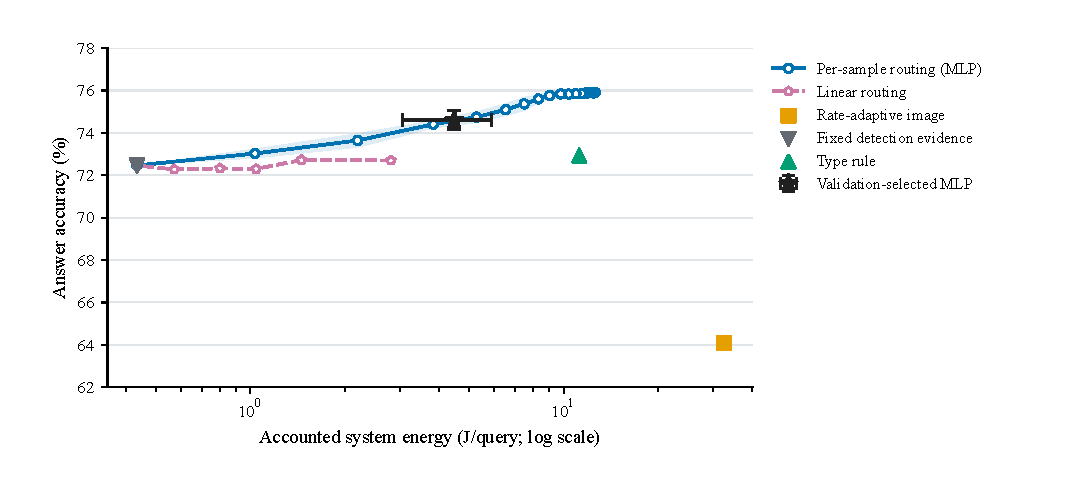
\includegraphics[width=\linewidth]{figures/evidence_final/dv_tradeoff.pdf}
\caption{DroneVehicle accuracy--energy trade-off over all $26$
fixed prices. The MLP curve gives ten-seed means at each price,
with shading for one sample standard deviation in accuracy.
The star averages seed-specific validation-selected points; its
error bars show one sample standard deviation in each coordinate.
It need not lie on the mean fixed-price curve. Energy is on a
logarithmic axis.}\label{fig:f5}
\end{figure}

\emph{System energy versus UAV energy.}\label{subsec:boundary}
Figure~\ref{fig:estack} separates the two platforms. Avoiding edge
VLM calls explains most of the reduction in total energy.
The priced MLP uses approximately $4.47$\,J in total, of which
$0.45$\,J is assigned to the UAV and $4.02$\,J to edge inference.
For fixed-image transmission, the UAV account is only $0.13$\,J
and the edge account is $32.31$\,J. The type rule's UAV cost is
$0.33$\,J. Thus, in this reference configuration, both routing
policies reduce system energy but increase modeled UAV energy
relative to fixed images. The claimed benefit is joint communication
and inference efficiency, not a demonstrated increase in flight time.

\begin{figure}[t]\centering
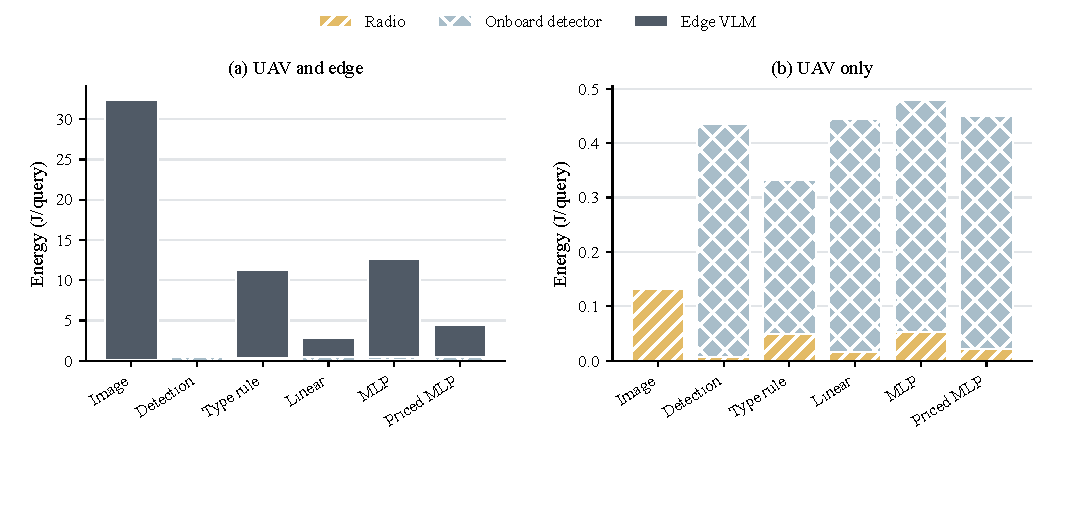
\includegraphics[width=\linewidth]{figures/evidence_final/dv_energy_components.pdf}
\caption{DroneVehicle energy components at the reported operating
points. The right panel excludes edge inference. MLP columns use
mean components over ten seeds. Detector and radio energy are
modeled; edge energy uses the fixed measured proxy. Excluded
components are stated in the experimental setup.}\label{fig:estack}
\end{figure}

\subsection{Receiver Adaptation}\label{subsec:crossvlm}\label{subsec:routerrobust}
We compare Qwen2-VL-2B, Qwen2.5-VL-3B, and SmolVLM using identical
paired question/SNR keys and byte-identical received images.
The shared detector records and training-only count calibration
are the same for all three receivers. The common partitions contain
$9{,}150/2{,}646/2{,}808$ training/validation/test decisions.
Each receiver has a separately fitted linear router and ten MLP
seeds with the same training settings. We also freeze the MLP
trained for Qwen2-VL on this common training set and apply its
unchanged decisions to the other receivers.

\begin{table}[t]\centering
\caption{Matched-receiver accuracy (\%), $\lambda=0$.
MLP entries are ten-seed means $\pm$ sample standard deviations.
Frozen-source routing uses the Qwen2-VL router without target-receiver
fitting.}\label{tab:crossvlm}
\footnotesize
\begin{tabular}{@{}lrrr@{}}\toprule
Policy & Qwen2-VL & Qwen2.5-VL & SmolVLM\\\midrule
Image & 62.93 & 62.57 & 59.29\\
Detection evidence & 67.09 & 67.09 & 67.09\\
Type rule & 69.34 & 67.31 & 67.38\\
Linear, receiver-specific & 69.59 & 68.38 & 68.13\\
MLP, receiver-specific & $69.63\pm0.38$ & $68.62\pm0.28$ & $69.29\pm0.57$\\
MLP, frozen source & --- & $68.28\pm0.43$ & $67.09\pm0.90$\\
\bottomrule\end{tabular}
\end{table}

Table~\ref{tab:crossvlm} shows that the MLP-minus-linear mean
accuracy differences are $0.04$, $0.25$, and $1.16$ points,
respectively. Receiver-specific fitting is therefore more useful
for some receivers than others. Freezing the Qwen2 router reduces
SmolVLM accuracy by $2.20$ points relative to its own MLP fit.
This supports adaptation to the answering mechanism, not arbitrary
receiver-independent routing.

The common test set includes $104$ images, but presence and counting
cover only $26$ of them. The other three types cover all $104$.
Consequently, these pooled accuracies cannot be compared directly
with the full VisDrone workload. The complete-five-type image
subset is reported separately in the supplementary materials.
No alternative-receiver energy measurements are available, so this
comparison reports accuracy and branch use, not energy savings.

\subsection{Discussion and Limitations}\label{sec:limits}
The results support question-conditioned evidence selection as a
joint choice of communication content and answering computation.
A fixed rule already captures useful differences between question
types. Per-sample prediction offers additional operating points,
but its benefit depends on the dataset, receiver, and cost assigned
to image inference. Small gains over a linear reference do not
justify a general claim for nonlinear routing.

The evaluation is limited to generated structured questions over
a modest aerial-image pool. Questions and SNR replays share images,
and image-disjoint splits do not establish independence between
nearby scenes. DroneVehicle uses only Rician and its router is
fitted on target training data. The matched-receiver workload has
unequal coverage across question types. These experiments do not
establish unrestricted-language performance or zero-shot transfer
to another aerial dataset.

Energy combines an edge-device measurement with modeled onboard
and radio costs. It assumes unbatched, per-question processing and
does not amortize detection across questions sharing an image.
The compact detection airtime and reference-window outage model
are not a validated finite-length wireless link. Source encoding,
radio circuitry, and several computation costs remain outside the
account. These assumptions limit deployment claims even when an
offline policy has lower modeled system energy. Embedded-device
measurements and online evaluation are needed to assess practical
latency and UAV battery effects.

\section{Conclusion}\label{sec:conc}
This paper presented an evidence-level routing system for structured
aerial VQA that jointly selects the transmitted representation and
the receiver's answering computation. A question-type rule exploits
differences in evidence requirements, while per-sample correctness
prediction and an energy price adjust the accuracy--energy trade-off.
On VisDrone, the type rule improves accuracy over fixed-image
transmission and reduces accounted system energy by about $55\%$
across three channel models. On DroneVehicle, the validation-selected
MLP improves accuracy by $1.67$ percentage points and reduces
accounted system energy by $60.1\%$ relative to the type rule.
The benefit of learned routing depends on the dataset and receiver;
nonlinear prediction is not uniformly better than a linear baseline.
These findings support matching both communication content and
receiver computation to the question, with energy savings arising
mainly from avoiding VLM inference when detection evidence is sufficient.
The savings apply to the evaluated UAV-and-edge energy model and
do not imply lower UAV energy, since onboard detection can outweigh
radio savings. Future work will evaluate end-to-end energy and
latency for online routing on embedded platforms.

% Appendix folded into §VI (reproducibility paragraph) for the 30-page
% TGCN review limit; 09_appendix.tex retained on disk but not \input.

% --------------------------------------------------------------------------
% References (single-spaced; body text remains double-spaced)
% --------------------------------------------------------------------------
\begin{singlespace}% IEEE-style smaller reference type (page budget):
% IEEEtran's thebibliography forces \footnotesize internally, so remap it
% to \scriptsize inside this group only.
\renewcommand{\footnotesize}{\scriptsize}%
\bibliographystyle{IEEEtran}
\bibliography{refs}
\end{singlespace}

\end{document}
